% Vẽ lại tín hiệu và các chú thích trong hình mẫu.
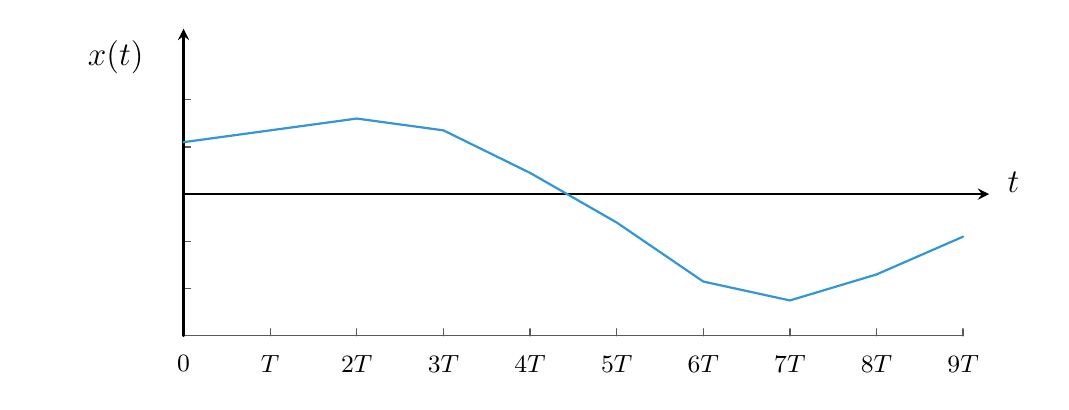
\begin{tikzpicture}[
    x=1.1cm,
    y=6cm,
    font=\small,
    line cap=round,
    line join=round
]
    % Cùng bề rộng với hình lấy mẫu để các mốc thời gian thẳng hàng.
    \path (-1.8, 0) -- (9.9, 0);
    \definecolor{analogsignal}{RGB}{50, 150, 215}

    % Đường chuẩn phía dưới và các vạch chia.
    \draw[black!65, line width=0.45pt] (0, -0.3) -- (9, -0.3);
    \foreach \position in {0,...,9} {
        \draw[black!65, line width=0.45pt]
            (\position, -0.3) -- (\position, -0.285);
    }
    \foreach \level in {-0.3, -0.2, -0.1, 0, 0.1, 0.2} {
        \draw[black!65, line width=0.45pt]
            (0, \level) -- (0.08, \level);
    }

    % Trục biên độ và trục thời gian.
    \draw[->, >=stealth, line width=0.8pt] (0, -0.3) -- (0, 0.35);
    \draw[->, >=stealth, line width=0.8pt] (0, 0) -- (9.3, 0);
    \node[anchor=east, font=\large] at (-0.35, 0.29) {$x(t)$};
    \node[anchor=west, font=\large] at (9.4, 0.025) {$t$};

    % Mốc thời gian theo các chú thích viết tay trên hình mẫu.
    \node[anchor=north] at (0, -0.32) {$0$};
    \node[anchor=north] at (1, -0.32) {$T$};
    \foreach \position in {2,...,9} {
        \node[anchor=north] at (\position, -0.32) {$\position T$};
    }

    % Các điểm biên độ được ước lượng từ ảnh, nối bằng đoạn thẳng.
    \draw[analogsignal, line width=0.8pt]
        (0, 0.11) -- (1, 0.135) -- (2, 0.16) -- (3, 0.135)
        -- (4, 0.045) -- (5, -0.06) -- (6, -0.185)
        -- (7, -0.225) -- (8, -0.17) -- (9, -0.09);

\end{tikzpicture}
